\documentclass[6pt]{article}
\title {DRAFT on ODE Coronavirus modeling}

\usepackage{graphicx}
\usepackage{amsthm}
\usepackage{amssymb}
\usepackage{amsmath}
\newtheorem{deff}{Definition}

\newcommand{\norm}[1]{\left\lVert#1\right\rVert}

\begin{document}
\maketitle
\section{Introduction}
A goal in modeling Coronavirus spreading is to describe the dynamic in 
time $t$ of the number of infected people $Y(t)$.
By taking its derivative one obtains the curve of the new infected,
ofter a quantity of interest, too.
Alternatively one might consider the numbers of deads, but we currently
aim at the former leaving the latter for future works.
Many models are available in the literature, but must of them belong to the
class of ODE interpolation. This is for instance the case for SIR, its
variants, as well as for many (generalized or not) logisic maps.

We start with a recap of two models, the Gompertz law and the classical
(basic) logistic map, that, despite their simplicity,
can give very effective results.

In practice one wants to estimate the parameters governing these ODEs,
starting from a dataset. When dealing with real data one can only estimate
the interpolation error. How to guess the true error from that, also
in the presence of noised measurements, is the topic of the following
section. Some issues are pointed out, like the need of a form of
injectivity and a generalized Lipschitz coefficient.

After a general introduction to the notion of Bayesian Inverse Problem,
such a method it is adapted to the current setting and proposed as a numerical
solution to the problems explained above, as well as as interpolation tool. 


In practice one work with datasets spanning from some day $1$ until $T$.
A naive approach would be to use the full range of data to test a model.
We clarify how this strategy might cause errors and point out a simple
criteria for finding a day $K$ to be considered as a better beginning time.
As we explain later, $K$ must satisfy at the same time a \emph{forward} and
a \emph{backward} stability property. If such a day does not exist,
then the ODE model should be considered inadequate, or the number of
obervations just too small.


Finally we apply all these results to perform predictions for Germany,
Italy and China via the Gompertz and Logistic maps. Extensions to other
ODEs are planned, since the principles exposed above can be easily adapted.


\section{Two simple models}
Altought the observations in this script can be applied, in principle,
to any kind of 1-dimensional ODE (generalizations are planned), we describe
now two specific models which we'll work out in detail
aiming to offer concrete examples and predictions.
Despite their simplicity, the proposed equations can be very effective.

Intuitively speaking both are S-shaped curves depending on two 
parameters, $\alpha$ and $N$. Usually
$\alpha \in (0, 1)$ and describes the slope of the S, while $N$ is the
asymptotic limit of infected people. Once $\alpha$, $N$ and the initial
conditions $N_0$ at time $t_0$ are fixed, the Gompertz Law is the solution to

\begin{equation}
\frac {dY (t)} {dt} = \alpha Y(t) \log[\frac{N} {Y(t)} ]
\end{equation}

while the Logistic map solves the ODE:
\begin{equation}
\frac {dY (t)} {dt} = \alpha Y(t) ( 1 - \frac{Y(t)}{N})
\end{equation}

Simple closed-form solutions are available, being

\begin{equation}
Y(t) = N \exp[ \log [ \frac{N_0}{N} \exp[-\alpha (t - t_0)]]]
\end{equation}

for the Gompertz law, and

\begin{equation}
Y(t) = \frac{N_0 \exp[\alpha(t - t_0)]}
	{1-\frac{N_0}{N} (1-\exp[\alpha(t-t_0)])}
\end{equation}

for the logistic map.
For the entire script, when we mean "Gompertz / Logistic map from day $n$",
we always intend to set that day to be time $0$, therefore
in practice we'll always have $t_0 = 0$.
Both these equations are particular case of 
generalized logistic maps, whose analysis is planned for the future.
We stress how we do not \emph{require} the need of a close-form solution
for our analysis, but using them reduce the propagation of numerical
errors. We clarify in the next section their error-analysis when
the goal is to estimate $\alpha$ and $N$.


\section{The noised Lipschitz constant}
Let's call $x$ the parameters governing an ODE (e.g. $x = \{ \alpha, N\}$
in the case of the Gompertz/Logistic law). Given a fixed initial condition here
omitted, $t_0 = 0$, 
let $Y_x = Y_x(t)$ be the trajectory in time corresponding to $x$.
Let $\hat{x}$ (with corresponding trajectory $\hat{Y}_x = \hat{Y}_x(t)$)
be a new set of parameters.


If we wanted to estimate them from the observed trajectories, 
it would be useful to have an inequality of the form:
\begin{equation}
\norm{ x - \hat{x} } \leq M \norm{Y_x - \hat{Y_x} }
\end{equation}

for some (possibly constant) $M$ and suitable norms.
Note that in the case of ODEs this is \emph{not} the classical
Lipschitz continuity property for the solution's existence.


The mentioned property is often tacitly assumed, and corresponds
to the idea that given a trajectory there is only one set of parameters
capable of reproducing it (parameters's injectivity), so that
a small residual error $\norm{Y_x - \hat{Y}_x}$ 
corresponds to a small true error $\norm{x - \hat{x}}$.


Had we such a property in theory, would it not represent
a solution in practice. First of all we never observe the full
trajectory $Y_x$, but rather just a limited number of days $Y_x(t_i)$,
and furthermore
the measurements are subjected to some noise. Let $\eta$ be a centered
gaussian distribution, $\eta_1$ and $\eta_2$ two realizations of it.
Then we are more interested to the \emph{noised} Lipschitz coefficient, 
defined as the (hypothetical constant) $\hat{M}$ such that:

\begin{equation}
\norm{ x - \hat{x} } \leq \hat{M} \norm 
	{Y_x(t_i) + \eta_1 - \hat{Y}_x(t_i) - \eta_2}
\end{equation}
where now the two trajectories are observed only in time
$\{t_1, \dots, t_T\} $ (typical around 30-40 days) and perturbed by a random
noise.


Suppose now to know the value of $\hat{M}$ (we'll estimate that
later, numerically, for both the Gompertz and the Logistic case).
Let's fix some empirical trajectory $Y_x(t_i) + \eta_1$.
Note that if we had a parameter $\hat{x}$ such that
$\norm{Y_x(t_i) + \eta_1 - \hat{Y}_x(t_i) - \eta_2} \leq \epsilon$,
we could deduce $\norm{ x - \hat{x} } \leq \hat{M} \epsilon$,
therefore solving the problem of parameter estimation if the
value is small enough.


The goal of the next section is to propose a bayesian strategy
for finding good candidates $\hat{x}$.

\section {Inverse Bayesian estimation}
As a general formulation, the (continuous) inverse problem 
consists on having a known continous map
$G: \mathbb{R}^n \to \mathbb{R}^m$, an \textbf{unknown} 
input $x \in \mathbb{R}^n$ to be found from
a known \emph{observation} $y = G(x) + \eta$, where $\eta$ is a centered
gaussian random variable, called the noise, with some specified variance.

In other words we are interested in performing an indirected measure
(the value $x$) from a direct measure $y$ and the use of a scientific
model $G$.

A \emph{lot} of theoretical issues are here into play. To mention
few of them, the map $G$ might admit different preimages, none at all,
or the noise might send $y$ outside the range of $G$.

Some of these problems are circumvented by minimizing some distance
$\norm{G(x) - y}$ instead, but they might be
insufficient e.g. for cases where $G$ is not differentiable or not injective.

The \emph{bayesian} setting offers a way to overcome the mentioned issues
by taking a probabilistic viewpoint. Instead of looking for a specific
single point $x$, one considers a probabilty distribution "updated"
 according to the values of $y$ by the use of Bayes's theorem.

Let $\rho(x)dx$ be the density of a gaussian 
on $\mathbb{R}^n$ representing our initial belief
about $x$, called the \emph{prior}. 
For instance, if experience suggests a preimage of $y$ 
to be around the origin, we choose zero mean and small covariance.
If no information is available, we start with a high-covariance matrix.
Hints might come e.g. from numerical experiments, since
the prior influences the effectiveness of the algorithm.

Let $\eta(x)dx$ be the density of the noise (abuse of notation).
By combining the Bayes's formula
\begin{equation}
\mathbb{P}[x | y] = \frac{ \mathbb{P}[y | x] \mathbb{P}[x]} {\mathbb{P}[y]}
\end{equation}
and the equation $y = G(x) + \eta$, we find:
\begin{equation}
\mu (x) \doteq \mathbb{P}[x|y] = \frac{ \eta(y - G(x)) \rho(x)} {\mathbb{P}[y]}
\end{equation}
Since the value of $y$ is fixed, the denominator is just
the probability normalization constant. The new probability measure
$\mu$ on $\mathbb{R}^n$ is called the \emph{posterior} and represents
the best knowledge that we can conclude about $x$, updating our initial
belief $\rho$ with the observation of $y$.

A mathematically rigorous version of the formulaes above is available in
the paper AAA, but we rather insist on a key point:
the solution of the question "find a preimage of $y$ in the presence of noise"
lies now in the ability
of sampling from the posterior probability distribution.
We use pCN MCMC - ADD MORE INFORMATION.

\section{Bayesian Inversion to detect injectivyty}
Explain k-means, centroids, how to use them to check
injectivity. 

\section {Using Bayesian Inversion as interpolator}
Let's consider our ODE model, say the logistic map, from time $0$.
It depends on two parameters $\alpha, N$ and once they are fixed,
it produces a series of observations in time $0,...$ until $T$.
Call them $Y_{\alpha, N}(t)$.

We are interested in \emph{deducing} $\alpha$ and $N$ from the noised
observed values. This situation can be read as a Bayesian inverse problem 
just by setting 
$G : \mathbb{R}^2 \to \mathbb{R}^T$ as
$\alpha, N \mapsto Y_{\alpha, N} (0), \dots, Y_{\alpha, N} (T)$.

Note that the continuity of $G$, here assumed, is precisely the same issue
of TOADD-NUMBEROFPARAGRAPH. 

Therefore: injectivity og G can ne checked numerically,
the parameter $M$ can be deduced numerically.

Summing up, we have now a way to numerically validate important ODE error
properties (Lip, injectivity) and to perform parameter estimation.
Given a dataset, there is only one step remaining: how to choose
a subset of it correctly.

\section{Choosing a good subinterval}
Let $Y(t)$ be the solution of a chosen ODE, for instance a logistic map.
As a first step for the modeling, we are interested is understanding 
how to correctly use a datasets spanning for $T$ days, $[1, \dots, T]$.
Now we would like to point out how one should generally
look at a subinterval $[K, T]$ of the dataset instead of the full one.

To understand why, and to set a way to compute $K$, we start 
"defining" $D$ as the minimal number of $D$ays required to perform a 
"meaningful" interpolation. This notion is something not rigorous, should
be improved, but has a clear meaning:
if you use only, say, two days $K$, $K+1$, you cannot hope to have any 
reliable interpolation. In practice I found $D$ to be around $7$ days,
but it's heuristic 
(of course, working with China, Korea, and random-generated toy-models).

We move now on the notion of \emph{forward} stability.
This is an obvious propoerty, but to label it will help later.

\begin{deff}[forward stability]
A day $K_1$ is said to satify the forward stability if 
by increasing $n = 0, 1, 2, \dots$, the parameter estimation of $\alpha$ 
and $N$ on every right-increasing intervals $[K_1, K_1 + D + n]$, 
until reaching $[K_1, T]$, produce the same results 
(up to approximation errors, of course).
\end{deff}

Note that for $n = 0$ we have the minimum amount of days in which we 
consider the interpolation to be meaningful.

The property before is considered always understood
and valid for every statistical interpolation. Conversely,
in our cases we deal specifically with ODEs. It means that they
satify the common start-and-stop property: running the dynamics
until time $T$ is the same as stopping it to time $K$, then
solving the ODE on $[K, T]$ with starting conditions $Y(K)$.

In other words, if an ODE is truly governing the process under observation,
no matter if we perform the estimation on $[1,\dots,T]$, or on any
$[n, T]$ (with new initial conditions),
the results must be the same since the parameters governing the
dynamic are always the same!
It leads to the notion of \emph{backward} stability.

\begin{deff}[backward stability]
A day $K_2$ is said to satify the backward stability, if
the parameter estimated on $[K_2, T]$ are the same on every
left-decreasing interval $[K_2 + n, T]$ 
(with $K_2 + n + D < T$, i.e. leaving enough days to allow a meaningful interpolation).
\end{deff}

Summing up, we say thay a day $K_1$ is forward-stable if the esimation
are the same on all the increasing intervals $[K_1 +n, T]$.
This is a generally valid statistical requirement.
Conversely, to control if a point $K_2$ satisfies backward stability we 
look from "now", time $T$, back to $K_2$, than back to $K_2 + 1$, etc...
This is a requirement coming from the usage of ODEs.

We obtain as a corollary:
if we want to model and ODEs on some dataset $[K, T]$, then $K$ must
satisty at the same time both the forward and the backward stability.


\section{Numerical experiments}

\subsection {Description of the approach}
As explained in section ADD, in order to estimate the true paramter error
from the interpolation one, we need to know the value of the noised
Lipshitz constant $\hat{M}$ for both the Logistic and the Gompertz laws, 
a constant whose
existance is of course not guaranteed.
We start observing that the typical dataset is composed 
by a number of observations
between $10$ and $40$ days, with a starting ODE conditions varying from $20$ to
$100$. The parameter $\alpha$ is between $0$ and $1$, while $N$ from $5000$
to an hypothetical $500000$ (maximum number of infected).
The noise on the data, i.e. the noise on the constant $\hat{M}$
must be of course the same used for the bayesian algorithm.
We choose a centered gaussian
$\eta$ with a diagonal covariance matrix, whose 
$i-th$ value is set to be equal to the measurement
$y$ at time $i$. In other words, each single measure it perturbed with a
variance equal to itself. The result is a more relevant error for smaller,
initial measurements, and a less relevant one for measurements later in time.
This is an attempt to model the idea that the more the time runs,
the better are the estimations since more attention to the problem
is showed. This is of course
an arbitrary choice, but we kept it since the obtained results are
encouraging.


Now that all the ingredients are prepared, we point out how we performed
millions of simulations with uniformly random parameters in the range
described above. We generating therefore toy-models data close to a realistic
observation, and used them to: perform a bayesian interpolation,
to see if in practice the algorithm is effective, estimate the noised constant
$\hat{M}$, study the probabilistic distribution of the samples (k-means).
The common results are:
\begin{itemize}
	\item both with the Logistic and the Gompertz law, the set of the
		sampled estimated parameters can be well approximated
		with a single centroid, if we consider two significative
		digits both on $\alpha$ and $N$. In other words,
		the interpolation, i.e. the map $G$, is
		"sufficiently injective";
	\item the noised constant $\hat{M}$ exists and has a stable
		probabilistic behavior.
\end{itemize}
Therefore we can trust the estimated parameters when done with real data,
and we can formulate a probabilistic range of parameters error
by only looking at the interpolation one. This is extremely good.

\subsection{Predictions for Italy and Germany}
Both the Italian and the German dataset relates the days to the number
of infected. For Italy the day $1$ is set to be the 20th of February,
while for Germany is considered to be the 25th of February.
Both run until the 30th of March, for a total of $40$ days for Italy
and $35$ for Germany.
Dealing with the models' properties, we found that for the logistic ODE:
\begin{itemize}
	\item $P[ \hat{M} < 1.000000e+04 ] = 9.999040e+01\%$
	\item $P[ \hat{M} < 1.000000e+03 ] = 9.671792e+01\%$
	\item $P[ \hat{M} < 1.000000e+02 ] = 8.093366e+01\%$
	\item $P[ \hat{M} < 1.000000e+01 ] = 5.564246e+01\%$
\end{itemize}
For the gompertz ODE, we found that the noised constant $\hat{M}$
has a \emph{surprisingly} much stable behavior, indeed:
\begin{itemize}
	\item $\mathbb{P}[ \hat{M} < 1.000000e+04 ] = 9.999984e+01\%$ 
	\item $\mathbb{P}[ \hat{M} < 1.000000e+03 ] = 9.992422e+01\%$ 
	\item $\mathbb{P}[ \hat{M} < 1.000000e+02 ] = 9.932928e+01\%$ 
	\item $\mathbb{P}[ \hat{M} < 1.000000e+01 ] = 9.635792e+01\%$ 
	\item $\mathbb{P}[ \hat{M} < 1 ] = 8.851800e+01\%$
\end{itemize}

The last value shows how the Gompertz equation is likely to posses
contraction properties. This is strong and helps reducing the
errors a lot.
When we move on real data, a necessary step is to compute the
value of $K$ as explained in paragraph.

\begin{figure}
  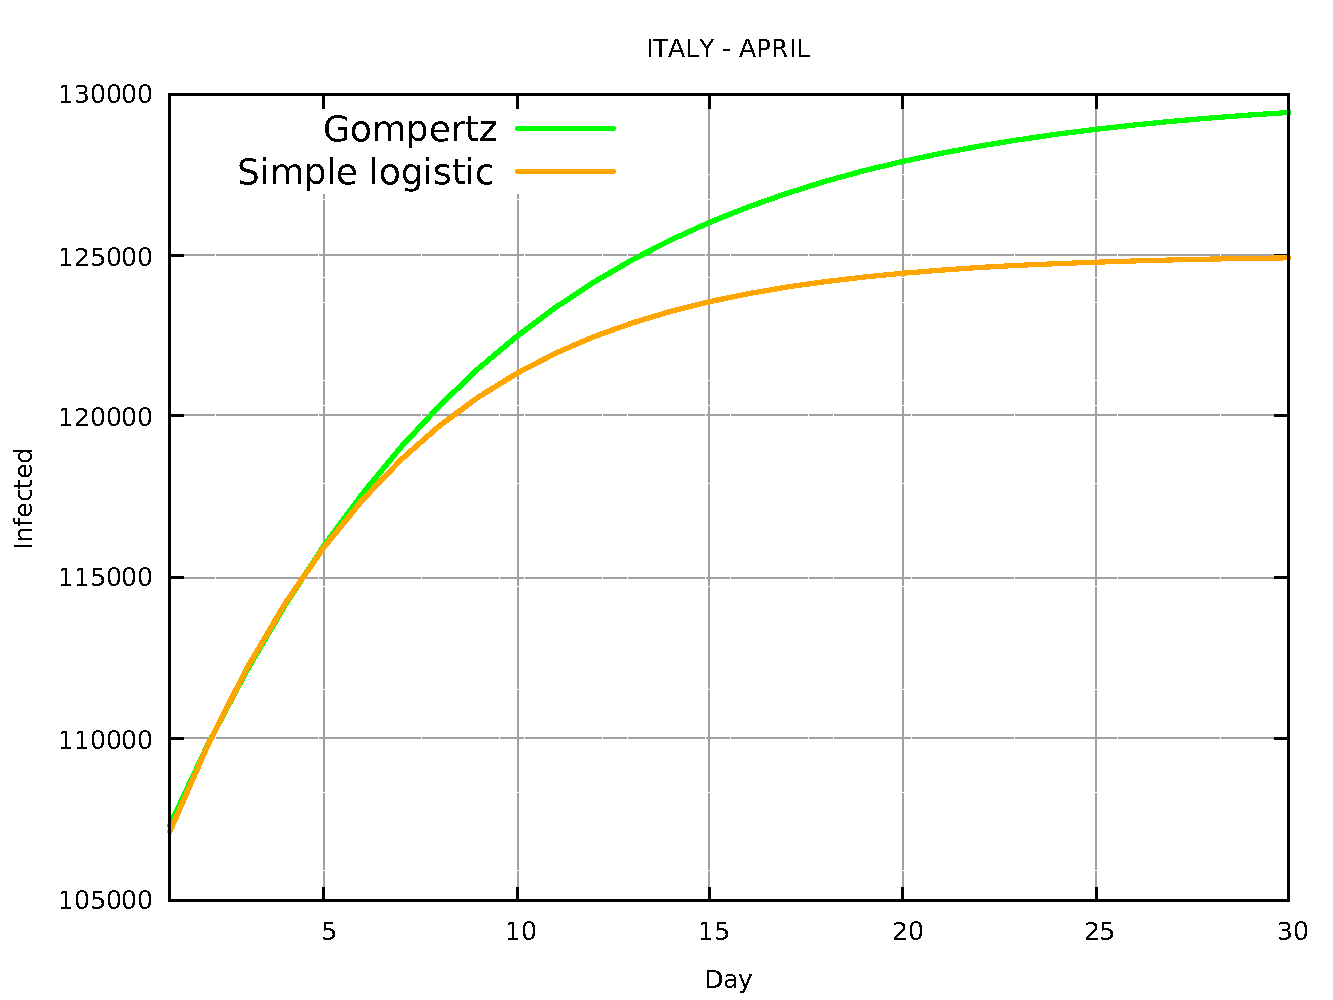
\includegraphics[width=\linewidth]{smaller_plot_april_italy.pdf}
  \caption{Predictions for April}
  \label{fig:boat1}
\end{figure}

\begin{figure}
  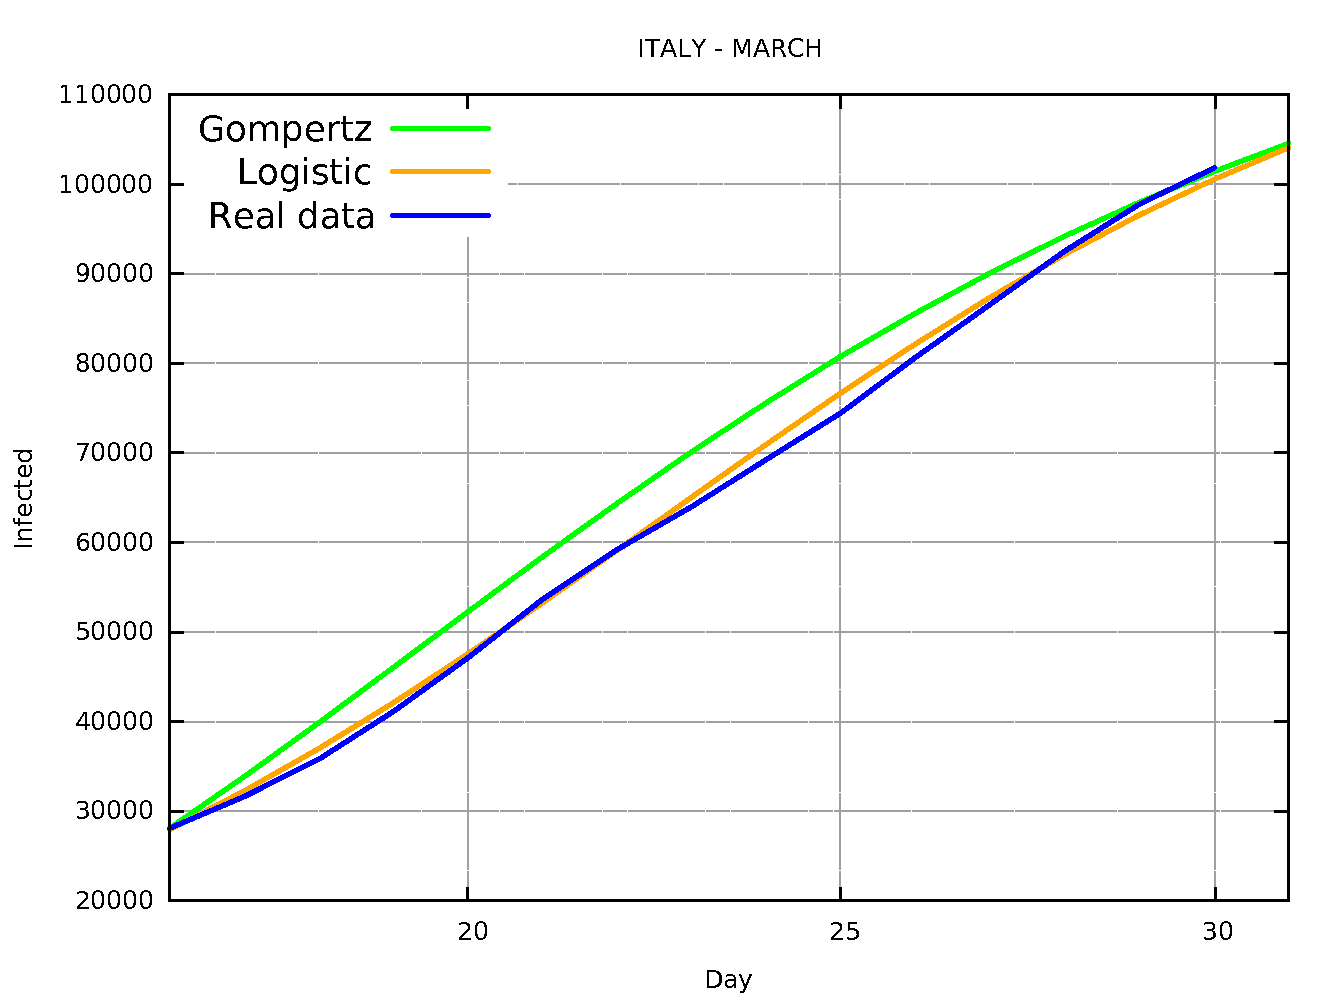
\includegraphics[width=\linewidth]{plot_march_italy.pdf}
  \caption{Interpolation on the current data in March}
  \label{fig:boat1}
\end{figure}


\subsubsection{Logistic predicion: Italy}
The found $K$ seems to be day $21$, corresponding to the 10th of March.
The estimated logistic parameters are $\alpha = 0.19$ and $N = 125000$
with a residual relative error of $1.54\%$,
absolute of around $4200$.

Attached is the plot showing real data VS logistic in March.
The second plot is the prediction for April.

In the plot we put these parameters, BUT, warning:
since $0 < \alpha < 1$ the residual error says to us not so much about
it, rather we can conclude, multiplying with $\hat{M}$, that the
maximum number of infected will not overclass $125000 + 4200 * 10 < 170.000$
with a probability higher than $55\%$ (see the table of $\hat{M}$ above).

\subsubsection {Logistic prediction: Germany}



\subsubsection{Gompertz predicion: Italy}
When using the Gompertz model for Italy, to find a clear value for $K$ is
harder. Indeed, the parameter $\alpha$ seems to stabilize around $0.11$
on $[21,40]$, but then slowly increase until $0.16$ on $[33,40]$.
Is it conversely very nice to see $N$ to be always close to $130000$
without any strong variation. 

Said that a more careful analysis must be done to be sure about the
parameter stabilization, we chose $K = 26$ with $\alpha = 0.13$, $N=13000$
and an absolute residual error around $10000$. It allows to claim that
with a probability of $88\%$ the number of infected will not
be higher than $130000 + 1.0 * 10000 = 140000$.
Variantions on $\alpha$ makes harder to establish clearly when this peak
is reached. The choice $\alpha = 0.13$ must be calibrated again 
when new data becomes available.

\subsubsection {Gompertz prediction: Germany}


\section {Conclusions}
\end{document}
